\documentclass[hyperref,pdfa,unicode,utf8,usepdftitle]{beamer}

\usepackage[l2tabu,orthodox,experimental]{nag}
\usepackage{cmap}

% \usepackage[english=]{csquotes}
\usepackage[USenglish]{babel}
\usepackage[utf8]{inputenc}
\usepackage[T1]{fontenc}
% \usepackage{indentfirst}
\usepackage{booktabs}
\usepackage{csquotes}
\usepackage{graphicx}
\usepackage{listings}
\usepackage{ragged2e}
\usepackage{siunitx}
\usepackage{tikz}
\usepackage{url}

% \usepackage{paralist}
% % https://tex.stackexchange.com/questions/255118/the-paralist-package-does-not-work-properly-in-beamer
% \newcommand{\paraitem}[1][1]{%
%  \quad
%  \makebox[\labelwidth][r]{%
%  \makelabel{%
%    \usebeamertemplate{description \beameritemnestingprefix item}}}%
%    \1\hskip\labelsep}

\usepackage{microtype}
\UseMicrotypeSet[protrusion]{basicmath}

% \usepackage{lmodern}
\usepackage{newtxtext}
\usepackage[straightquotes]{newtxtt}
\usepackage{hyperref}

\definecolor{meteosystemdefault}{rgb}{0.5,0.08,0.08}

\setbeamertemplate{footline}[frame number]
\setbeamerfont{page number in head/foot}{size=\large}
\setbeamertemplate{navigation symbols}{}
\AtBeginSection{\frame{\sectionpage}}

\usetikzlibrary{fit}
\usetikzlibrary{positioning}

\lstset{language=csh}
\lstset{basicstyle=\ttfamily\color{green!40!black}}
\lstset{upquote=true}

%%%%%%%%%%%%%%%%%%%%%%%%%%%%%%%%%%%%%%%%%%%%%%%%%%%%%%%%%%%%
% Document content start

\title{Meteo Student Linux Workshop}
\institute{Penn State Department of Meteorology and Atmospheric Science}
\author{PSU Weather Data Science Club}
\subject{An introduction to Unix, Linux, and the shell}
\titlegraphic{\includegraphics[width=0.5\textwidth]{linux-penguin}}

\begin{document}
\begin{frame}
  \titlepage{}
\end{frame}

\begin{frame}
  \frametitle{Acknowledgments}
  This presentation would not have been possible without Shawn
  Murdzek’s work putting this together for the graduate students last
  year (2021).

  This work is licensed under the Creative Commons Attribution 4.0
  International License. To view a copy of this license, visit
  \url{http://creativecommons.org/licenses/by/4.0/}.
\end{frame}

\begin{frame}
  \frametitle{Workshop Overview}
  \begin{description}
  \item[Goal] Teach the basics of working on the PSU METEO Linux
    network using the terminal
  \item[Prerequisite Knowledge] You've used a computer before and have
    some experience with Windows or Mac OS
  \item[Structure] Two forty-five-minute sessions with a ten-minute break in between
  \end{description}

  \begin{tabular}{ll>{\RaggedRight\arraybackslash\noindent}p{5cm}}
    45 min. & What is Linux? & Terminology, basic principals, and basic commands \\
    10 min. & Break \\
    45 min. & Hands-on Exercises & More advanced commands, running code \\
  \end{tabular}
  % \begin{columns}
  %   \begin{column}{7em}
  %     45 min. \\
  %     10 min. \\
  %     45 min. \\
  %   \end{column}
  % \end{columns}
\end{frame}

\section{What is Linux}

\begin{frame}
  \frametitle{Operating System}
  Handles hardware-software communication. The central part of the OS
  is called the \emph{kernel}

  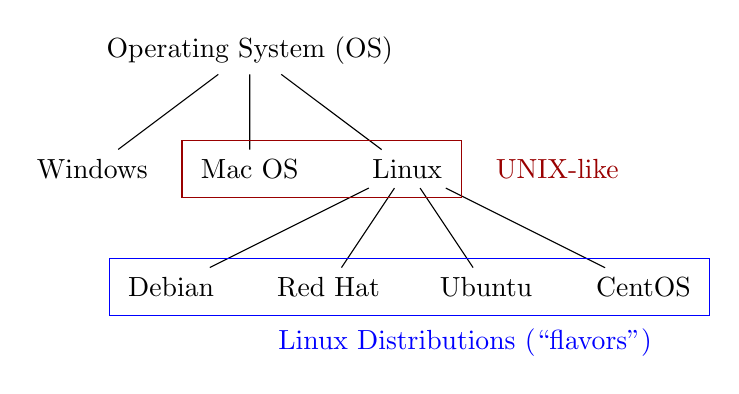
\begin{tikzpicture}[level 1/.style={sibling distance=2cm},level 2/.style={sibling distance=2cm}]
    \node{Operating System (OS)} %
      child { node {Windows} }
      child { node (Mac OS) {Mac OS} }
      child { node (Linux) {Linux}
        child { node (Debian) {Debian} }
        child { node (Red Hat) {Red Hat} }
        child { node (Ubuntu) {Ubuntu} }
        child { node (CentOS) {CentOS} }
      };
      \node[draw,fit=(Mac OS) (Linux),red!60!black] (unix box) {};
      \node[right of=Linux,anchor=west,red!60!black] {UNIX-like};
      \node[draw,blue,fit=(Debian) (Red Hat) (Ubuntu) (CentOS)] (linux-dists) {};
      \node[below right of=linux-dists,blue] {Linux Distributions (``flavors'')};
  \end{tikzpicture}
  \begin{itemize}
  \item Linux is a popular choice for supercomputers (e.g., PSU Roar,
    NCAR Cheyenne)
  \item One of the benefits of Linux is that it is \emph{open source}, which
    means the kernel is free and people can tinker with it
  \end{itemize}
\end{frame}

\begin{frame}
  \frametitle{Some Computer Jargon}
  \begin{description}
  \item[Server]  Any device (e.g., computer) that processes
    requests made by clients
    \begin{itemize}
    \item Ex) Web servers deliver website information to users when
      surfing the internet
    \item Ex) Cloud servers are remote computers that can be accessed
      over the internet
    \end{itemize}
  \item[Cluster]  A collection of computers used to perform
    computationally-intensive tasks
    \begin{itemize}
    \item Ex) NCAR Cheyenne supercomputer
    \end{itemize}
  \item[Node] A single device in a larger network (e.g., server,
    printer, desktop)
  \item[Central Processing Unit (CPU)] Can refer to the computer chip
    (e.g., Intel i7) or the number of cores (each core can handle one
    process)
    \begin{itemize}
    \item “Core,” “CPU,” and “processor” tend to be used
      interchangeably
    \item See slides at the end of this presentation for a deeper dive
      on this topic
    \end{itemize}
  \item[Parallelization]  Dividing a task between multiple cores for
    increased efficiency
    \begin{itemize}
    \item “Using a comb instead of a toothpick to comb your hair”
    \end{itemize}
  \end{description}
\end{frame}

\begin{frame}
  \frametitle{PSU Meteo Linux network}
  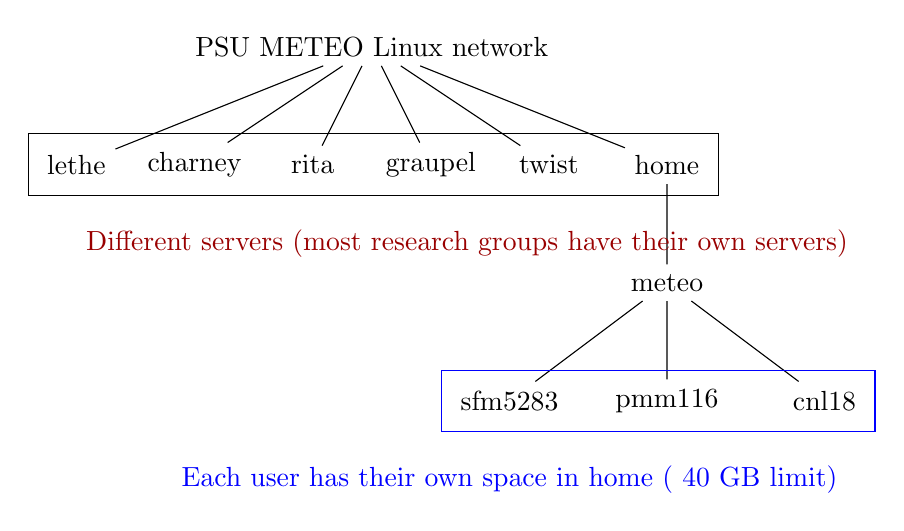
\begin{tikzpicture}[level 1/.style={sibling distance=1.5cm},level 2/.style={sibling distance=2cm}]
    \node {PSU METEO Linux network}
    child { node (lethe) {lethe} }
    child { node (charney) {charney} }
    child { node (rita) {rita} }
    child { node (graupel) {graupel} }
    child { node (twist) {twist} }
    child { node (home) {home}
      child { node (meteo) {meteo}
        child { node (sfm5282) {sfm5283} }
        child { node (pmm116) {pmm116} }
        child { node (cnl18) {cnl18} }
      }
    };
    \node[draw,fit=(lethe) (charney) (rita) (graupel) (twist) (home)] {};
    \node[below of=lethe,anchor=west,red!60!black] {Different servers
      (most research groups \breakhere have their own servers)};
    \node[draw,fit=(sfm5282) (pmm116) (cnl18),blue] {};
    \node[below of=sfm5282,blue] {Each user has their own space in home (~40 GB limit)};
  \end{tikzpicture}
  In addition to the space allotted on home, students typically have
  large amounts of space on their research group’s server as well.

  PSU METEO servers live on the sixth floor in a sealed room.
\end{frame}

\begin{frame}
  \frametitle{GUI vs. CLI}
  \begin{columns}
    \begin{column}{0.5\textwidth}
      \textbf{Graphical User Interface:} User interacts with computer
      using graphics.  The program in charge of displaying graphics
      and sending input is the X server.  GUIs are often more user
      friendly, but generally slower and less precise
    \end{column}
    \begin{column}{0.5\textwidth}
      \textbf{Command Line Interface:} User interacts with computer
      using typed commands. Harder to use, but generally faster and
      more efficient (UNIX CLI is called “the shell”)
    \end{column}
  \end{columns}
\end{frame}

\subsection{Connecting to the PSU Meteo Linux Network}

\begin{frame}
  \frametitle{Connecting to the PSU Meteo Linux Network}
  \begin{description}
  \item[Windows] Prior to Windows 10, PCs could not connect to Linux
    servers on their own. Instead, they used a third-party terminal
    emulator (e.g., MobaXterm, PuTTY)
    \begin{itemize}
    \item Machines running Windows 10 can use ssh from the Windows
      command line
    \item Windows machines can also install MobaXTerm
      \begin{itemize}
      \item Install MobaXterm (see next slide)
      \item Click “Start local terminal”
      \item Type
        \lstinline{ssh abc1234@ulteosrv2.met.psu.edu}
      \item Authenticate
      \end{itemize}
    \end{itemize}
  \item[Mac] Can connect to Linux servers using the Terminal app
  \end{description}
  Note: All commands will be given in \lstinline{a monospace font} and
  placeholders will be underlined
\end{frame}

\begin{frame}
  \frametitle{Downloading MobaXterm on the Walker Workstations}
  \begin{itemize}
  \item Each user must download MobaXterm into their profile space
    \begin{itemize}
    \item The system administrator (Chad) can’t do this for us
    \item I recommend the Desktop folder, but V or X should work as
      well
    \end{itemize}
  \item Steps:
    \begin{itemize}
    \item Visit \url{https://mobaxterm.mobatek.net/download.html}
    \item Download the Home Edition (Portable Version)
    \item Copy zip file from Downloads into Desktop (or other desired
      location)
    \item Unzip zip file
    \item Double-click the application to run
    \item You’ll get a couple of warnings, just run anyways
    \end{itemize}
  \item I also recommend creating a shortcut and adding that to your
    home screen
  \end{itemize}
\end{frame}

\subsection{Interacting with the UNIX Shell}

\begin{frame}[fragile]
  \frametitle{The Shell: The UNIX CLI}
\begin{lstlisting}
lethe:sfm5282[766]% ls
\end{lstlisting}
  Server name, user name, line number, prompt, command
  \begin{itemize}
  \item Default shell for the METEO network is tcsh (enhanced UNIX
    Berkeley C shell)
  \item Other common shells: bash, ksh, zsh
  \item Basic functionality is nearly identical between the different
    shells
  \item Can switch to bash by simply running the
    command \lstinline{bash} (to go back to tcsh,
    run \lstinline{exit})
  \end{itemize}
\end{frame}

\begin{frame}[fragile]
  \frametitle{Linux commands: syntax}
\begin{lstlisting}
command [options] [arguments]
\end{lstlisting}
  % \lstinline[emph={options},emphstyle={\color{red!60!black}},emph={[2]arguments},emphstyle={[2]\color{blue}}]{command [options] [arguments]}

  % TODO: add descriptions for colors
  Try the following commands...
  \begin{tabular}{lp{3in}}
    \texttt{ls} & List storage \\
    \texttt{ls -{}-help} & Display the help page for \texttt{ls}. Most commands have this option \\
    \texttt{ls -l} & Same as \texttt{ls} but with the “long” option (shows more information) \\
    \texttt{man ls} & Display the documentation (manual) for \texttt{ls}
  \end{tabular}
\end{frame}


\begin{frame}
  \frametitle{Moving around a Linux system}
  \begin{columns}
    \begin{column}{0.3\textwidth}
      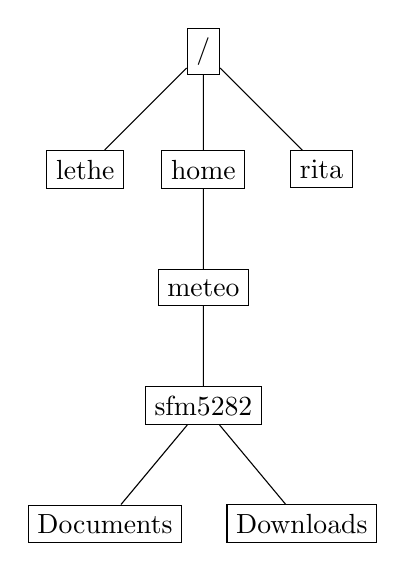
\begin{tikzpicture}[level 4/.style={sibling distance=2.5cm}]
        \node[draw] {/}
        child { node[draw] {lethe} }
        child { node[draw] {home}
          child { node[draw] {meteo}
            child { node[draw] {sfm5282}
              child { node[draw] {Documents} }
              child { node[draw] {Downloads} }
            }
          }
        }
        child { node[draw] {rita} };
      \end{tikzpicture}
    \end{column}
    \begin{column}{0.6\textwidth}
      \begin{itemize}
      \item \textbf{File Tree:} Layout of folders (shown on right)
        \begin{itemize}
        \item \lstinline{pwd} prints your location in the file tree 
        \end{itemize}
      \item Changing directories (command: \lstinline{cd})
        \begin{itemize}
        \item \lstinline{cd /} (move to root directory)
        \item \lstinline{cd /home/meteo/abc1234/Documents}
        \end{itemize}
      \item \textbf{Absolute Path:} Full path name
      \item \textbf{Relative Path:} Path is relative to current
        directory
        \begin{tabular}{ll}
          \texttt{.} & Current level \\
          \texttt{..} & Up one level \\
          \texttt{\~} & Home directory
        \end{tabular}
      \end{itemize}
    \end{column}
  \end{columns}
\end{frame}

\begin{frame}
  \frametitle{Creating and Removing Directories}
  \begin{itemize}
  \item \lstinline{mkdir} makes a directory, \lstinline{rmdir} removes
    an empty directory
  \item Try the following
    \begin{itemize}
    \item \lstinline{cd ~}
    \item \lstinline{mkdir test}
    \item \lstinline{ls} (this should show a new directory)
    \item \lstinline{rmdir test}
    \item \lstinline{ls}
    \end{itemize}
  \end{itemize}
\end{frame}

\begin{frame}
  \frametitle{Create a Sample Directory and Sample Files}
  \begin{itemize}
  \item \lstinline{cd ~}
  \item \lstinline{mkdir test_dir}
  \item \lstinline{cd test_dir}
  \item \lstinline{touch my_file}
  \item \lstinline{nano my_file} (add some text, WriteOut, then Exit)
  \item \lstinline{nano my_file2} (add some text, WriteOut, then Exit)
  \item \lstinline{file my_file2} (show file type, should be an ASCII
    text file)
  \end{itemize}

  Note that “\^X” means to hold down the control key (perhaps command
  on Mac), press “X”, then release both keys; this is also written
  “Ctrl-X”
\end{frame}

\begin{frame}
  \frametitle{Moving and Removing files}
  \begin{itemize}
  \item \lstinline{cd ~/test_dir}
  \item \lstinline{mv my_file ..} (move my\_file to parent directory
    with same name)
  \item \lstinline{cp my_file2 ..} (copy my\_file2 to parent directory
    with same name)
  \item \lstinline{ls ..} (List contents of parent directory)
  \item \lstinline{ls} (Defaults to \lstinline{ls .}; list contents of
    current directory)
  \item \lstinline{cd ..} (Change current directory to parent of current directory)
  \item \lstinline{rm my_file2}
  \item \lstinline{rm my_file}
  \end{itemize}

  \alert{Removing a file is forever! There is no undo or recycling bin!}

  Useful options for \lstinline{rm}:
  \begin{itemize}
  \item \lstinline{rm -r}: Remove all files and folders within a
    directory.  Be careful with this command.
  \item \lstinline{rm -i}: Ask for confirmation before deleting each
    file
  \end{itemize}
\end{frame}

\begin{frame}[fragile]
  \frametitle{\protect{\lstinline{ls -l}} Output}
\begin{lstlisting}
ulteosrv2:sfm5282[622]% ls -l
total 44
-rw-r--r--. 1 sfm5282 users 26768 Apr 16  2017 hwk9_prob17.pdf
-rw-r--r--. 1 sfm5282 users  2682 Apr 26  2017 math406_script.py
drwxr-xr-x. 3 sfm5282 users  4096 Feb 19  2018 math455
drwxr-xr-x. 2 sfm5282 users  4096 Sep 30  2020 math456
-rw-r-----. 1 sfm5282 users   675 Apr 28  2017 parametric.py
\end{lstlisting}
  \begin{itemize}
  \item File type (d = directory; - = regular file)
  \item File permissions (next slide)
  \item Number of hard links to file
  \item File owner
  \item File group
  \item File size (bytes; use \lstinline{-h} option to get
    ``human-readable'' units like megabytes or kilobytes as
    appropriate)
  \item Date last modified
  \item File name
  \end{itemize}

  % Explore the documentation
  % (\lstinline{ls --help}, \lstinline{man ls}, \lstinline{info ls}) to
  % find sort options and to change the units on file size.
\end{frame}

\begin{frame}
  \frametitle{Reading File Permissions}
  \begin{itemize}
  \item Three groups of three letters, each denoting a permission
    granted or denied
  \item The letters within each group (the first three are in order):
    % \begin{description}
    % \item[r] Read
    % \paraitem[w] Write
    % \item[x] Execute (files)/View contents (directories)
    % \paraitem[-] Permission not granted
    % \end{description}
      \begin{tabular}{l>{\RaggedRight\arraybackslash\noindent}p{4cm}l>{\RaggedRight\arraybackslash\noindent}p{4cm}}
      r & Read & w & Write \\
      x & {Execute~(files)} / view contents (directories) & - & Permission not granted
    \end{tabular}
  \item The groups represent permissions granted to the file owner,
    the file group, and to everyone else
  \item Example:

    
\begin{tikzpicture}
      \node (owner) {rwx};
      \node[right=0cm of owner] (group) {rw-};
      \node[right=0cm of group] (other) {r-{}-};
      \node[below left=0.14cm of owner] {Owner};
      \node[below=0.1cm of group] {Group};
      \node[below right=0.14cm of other] {Everyone else/other};
    \end{tikzpicture}
  \end{itemize}
\end{frame}

\begin{frame}
  \frametitle{Changing File Permissions}
  \lstinline{chmod permissions file}

  \begin{itemize}
  \item \lstinline{permissions} is a comma-separated list of groups
    and permissions to set (\lstinline{=}), add (\lstinline{+}), or
    remove (\lstinline{-}) for those groups
    % \begin{description}
    % \item[u] user/owner
    %   \paraitem[g] group
    % \item[o] others/everyone else
    %   \paraitem[a] all
    % \end{description}
    \begin{tabular}{l>{\RaggedRight\arraybackslash\noindent}p{4cm}l>{\RaggedRight\arraybackslash\noindent}p{4cm}}
      u & user/owner           & g & group \\
      o & others/everyone else & a & all
    \end{tabular}

    \item Examples
    \begin{itemize}
    \item \lstinline{touch test\_file}
    \item \lstinline{chmod u=rwx,g+r,o-x test\_file}
    \item \lstinline{ls -l}
    \end{itemize}
    \end{itemize}
\end{frame}

\begin{frame}
  \frametitle{The Module System}
  \begin{itemize}
  \item Used to load packages not installed by the standard Linux
    distribution, or to manage multiple versions of packages
  \item Example: Using IPython/Jupyter
    \begin{itemize}
    \item The default Python is older and does not have IPython
      installed (try running \lstinline{ipython} to check)
    \item \lstinline{module list} (Shows a list of the currently-loaded modules)
    \item \lstinline{module avail} (Shows all modules available to be loaded)
      \begin{itemize}
      \item Modules marked with \lstinline{(D)} are loaded by default
      \end{itemize}
    \item \lstinline{module spider python} (Show python modules that
      can be loaded)
    \item \lstinline{module load python} (loads most recent python
      module; can now run IPython)
    \item \lstinline{module swap python/3.7.6_anaconda} (Switch python
      module to use a different version)
    \item \lstinline{module purge} (Unloads all modules)
    \end{itemize}
  \end{itemize}
\end{frame}

\begin{frame}
  \frametitle{Aliases}
  \begin{itemize}
  \item Linux command shortcuts
  \item The Meteo network comes with many built-in aliases
    \begin{itemize}
    \item \lstinline{alias} with no arguments will print all defined
      aliases
    \end{itemize}
  \item You can make new aliases with \lstinline{alias name "command"}
    \begin{itemize}
    \item Aliases only last until the end of the current shell session
      (i.e., until you log out)
    \end{itemize}
  \item Example
    \begin{itemize}
    \item \lstinline{cd ~}
    \item \lstinline{mkdir dir1}
    \item \lstinline{mkdir dir1/dir2}
    \item \lstinline{alias dd "cd ~/dir1/dir2"}
    \item \lstinline{dd} (should move you into \lstinline{dir2}; try
      running in different directories)
    \end{itemize}
  \end{itemize}
\end{frame}

\begin{frame}
  \frametitle{Hidden files}
  \begin{itemize}
  \item \lstinline{ls} does not, by default, display files whose names
    begin with \lstinline{.}
  \item \lstinline{ls -a} will display all files, including those
    whose names start with \lstinline{.}
  \item \lstinline{.} is a special file indicating the current
    directory
  \item \lstinline{..} is a special file indicating the parent of the
    current directory
    \begin{itemize}
    \item the parent of \url{~/dir1/dir2} is \url{~/dir1}
    \end{itemize}
  \item Many hidden files in your home directory are configuration
    files read when some program starts
  \end{itemize}
\end{frame}

\begin{frame}
  \frametitle{Login files (\texttt{.cshrc.cat})}
  \begin{itemize}
  \item One useful hidden file is your shell configuration
    file \url{~/.cshrc.cat}, which the Meteo systems run when
    you start a new \lstinline{tcsh}
  \item Within this file, you can load modules, create aliases, and
    otherwise customize the shell to your liking
  \item Try the following:
    \begin{itemize}
    \item Add the line \lstinline{module load python} to
      your \url{~/.cshrc.cat}
    \item Open a new terminal (new tab on MobaXTerm) and log in to the
      Meteo servers
    \item The shell should load the python module for you as you log in
    \end{itemize}
  \item You might want to make \lstinline{rm} an alias
    for \lstinline{rm -i} in your \url{~/.cshrc.cat}
  \end{itemize}
\end{frame}

\begin{frame}
  \frametitle{Checking Storage Limits}
  \begin{itemize}
  \item Users have a limited amount of space in their home space
    \begin{itemize}
    \item Use the command quota to display how much space is used and
      how much is left
    \item Use the -s option to print the quota in human-readable units
    \end{itemize}
  \item Other useful commands:
    \begin{itemize}
    \item \lstinline{du} = Disk usage, estimates the amount of space each
      file/folder takes up
    \item \lstinline{du -h} = Human-readable units
    \item \lstinline{du -d x} = Max depth (= x)
    \item The output here is very long! You can write the output to
      a text file using du > file
    \item \lstinline{df} = Disk free, displays the amount of available space on
      the file system
    \item \lstinline{df -h} = Human-readable units
    \end{itemize}
  \end{itemize}
\end{frame}

\subsection{Editors and Interactive Development Environments}

\begin{frame}
  \frametitle{Exploring Other Text Editors: \texttt{vim}}
  \begin{itemize}
  \item Vim is less intuitive than nano, but it provides a lot more
    functionality than nano
  \item Vim has two main modes:
    \begin{itemize}
    \item Command: Similar to a CLI. Includes commands to move around
      a document, copy text, delete text, save your work, etc.
      \begin{itemize}
      \item Vim defaults to command mode when you open a document
      \end{itemize}
    \item Insert (edit): Allows the user to type text
    \end{itemize}
  \item Useful commands:
    \begin{itemize}
    \item \lstinline{i} = Switch to insert mode
    \item \lstinline{Esc key} = Switch back to command mode
    \item \lstinline{:w} = Save work (in command mode)
    \item \lstinline{:q} = Quit vim (in command mode)
    \item \lstinline{:q!} = Quit vim without saving (in command mode)
    \end{itemize}
  \end{itemize}
\end{frame}

\begin{frame}
  \frametitle{Editing and Running Code}
  \begin{itemize}
  \item Up to this point, we have only discussed command line tools
    \begin{itemize}
    \item To make life easier, there are various GUIs available
    \end{itemize}
  \item We can run, edit, and debug code on the Meteo servers
  \item Python
    \begin{itemize}
    \item Spyder \lstinline{spyder}
    \item JupyterLab\footnote{if you need help setting up JupyterLab,
        please contact Karl (\url{mailto:kps5442@psu.edu})} (many types of
      files) \lstinline{jupyter lab}
    \end{itemize}
  \item Matlab: \lstinline{matlab} (also has a CLI)
  \item Text editors: \lstinline{gvim}, \lstinline{emacs} (also has
    CLI), \lstinline{geany}, \lstinline{gedit}
  \end{itemize}
\end{frame}

\begin{frame}
  \frametitle{Running Code After Logging Out}
  \begin{itemize}
  \item \lstinline{nohup command} Creates an environment that ignores
    log-out signals, then runs \lstinline{command}
  \item \lstinline{screen} Creates an interactive session with a
    shell, then connects you to it
    \begin{itemize}
    \item Leave a screen session: Ctrl-A; D
    \item Resume a screen session: \lstinline{screen -r}
    \item Close a screen session: Ctrl-D
    \item List running screen sessions: \lstinline{screen -ls}
    \end{itemize}
  \item \lstinline{tmux} Like screen, but with different defaults and
    more setup remembered on resuming a detached session
  \item \lstinline{vncserver}/\lstinline{vncviewer}: Like screen for X
    applications/GUIs
  \item \lstinline{nice command} Decreases the process priority then
    runs \lstinline{command}.  Intended to keep other people's
    programs from freezing.
  \end{itemize}
\end{frame}

\subsection{Conclusions}

\begin{frame}
  \frametitle{Session 1: Key Take-home Points}
  \begin{itemize}
  \item Linux is an operating system typically used on
    high-performance computers
    \begin{itemize}
    \item The PSU METEO Network, as well as NCAR Cheyenne and PSU
      Roar, use Linux
    \end{itemize}
  \item The command line interface (CLI) provides a more precise and
    efficient way to work on a computer compared to graphical user
    interfaces (GUIs)
    \begin{itemize}
    \item The tradeoff is that the learning curve for the CLI is
      steeper
    \item Mastering Linux takes time! Try doing something in Linux
      every work day to get more comfortable
    \end{itemize}
  \item There are many different Linux CLI flavors. The METEO Network
    defaults to tcsh
  \item Using the CLI, we can do several things, including
    \begin{itemize}
    \item Creating, moving, copying, and deleting files and
      directories
    \item Adjusting file permissions
    \item Configuring our computing environment (e.g., load specific
      modules, create aliases, etc)
    \end{itemize}
  \item \alert{In the next session, we’ll run a program to analyze
      some radar data}
  \end{itemize}
\end{frame}

\section{Interactive Session}
\begin{frame}
  \frametitle{Task Overview}
  \begin{description}
  \item[Goal] Compute 1-km circulation around each gridpoint in a wind
    retrieval of an observed supercell thunderstorm
  \item[Materials] \url{linux_ws_exercise.tar.gz}
    \begin{itemize}
    \item This is a gzipped tarball that contains the wind retrieval
      and a fortran program to compute circulation
    \end{itemize}
  \item[Steps]
    \begin{itemize}
    \item Copy zipped tarball to METEO Linux Network and extract
      contents
    \item Load appropriate modules and create soft link for netcdf
      libraries
    \item Compile fortran program
    \item Configure input file and run fortran program
    \item Peruse results using ncview
    \end{itemize}
  \end{description}
\end{frame}

\subsection{Background}

\begin{frame}
  \frametitle{Compiled vs Interpreted Programming Languages}
  \begin{columns}
    \begin{column}{0.5\textwidth}
      \begin{center}
        \textbf{Compiled}
      \end{center}
      \begin{itemize}
      \item Source code is compiled into machine code (i.e., a
        binary), and the machine code is what is actually run
      \item Code must be recompiled each time it’s altered
      \item Machine code is platform dependent (i.e., it only works on
        the computer it’s compiled on)
      \item \textbf{Pros}: Tends to be faster than interpreted code
      \item \textbf{Examples}: C, C++, \alert{Fortran}, Go
      \end{itemize}
    \end{column}
    \begin{column}{0.5\textwidth}
      \begin{center}
        \textbf{Interpreted}
      \end{center}
      \begin{itemize}
      \item Source code is run by an interpreter, which runs the
        program line-by-line
      \item Code can be run on any computer that has an interpreter
        installed
      \item \textbf{Pros}: Generally easier to debug, more flexibility
        when changing computers, code is usually more readable
      \item \textbf{Examples}: Python, Matlab, Java, R, C shell
      \end{itemize}
    \end{column}
  \end{columns}
\end{frame}

\begin{frame}
  \frametitle{What is NetCDF?}
  \begin{itemize}
  \item Data format and supporting libraries developed by Unidata
    (part of UCAR)
    \begin{itemize}
    \item NetCDF = Network Common Data Format
    \item One of the most common data formats in meteorology
    \end{itemize}
  \item Designed to handle multi-dimensional datasets and metadata
    \begin{itemize}
    \item Metadata = Variable names, units, scaling, data source
      (model or instrument), experiment, etc.
    \end{itemize}
  \end{itemize}
\end{frame}

\subsection{Exercise steps}

\begin{frame}
  \frametitle{Copy zipped tarball and extract contents}
  \begin{itemize}
  \item (Inside \url{~} on Linux servers) \lstinline{mkdir linux_ws}
  \item (In Windows) Save \url{linux_ws_exercise.tar.gz} file
    in \url{Downloads} folder
  \item If you don’t have
    it:
    \url{https://github.com/DWesl/linux_ws_exercise/archive/refs/tags/v1.1.tar.gz}
  \item Open another MobaXterm tab, but don’t sign in
    \begin{itemize}
    \item Navigate to the folder on your Windows machine where you
      saved \url{linux_ws_exercise.tar.gz}
      \begin{itemize}
      \item On the Walker Desktops, this is
        likely
        \lstinline{cd C:/Users/abc1234/OneDrive\\ -\\ The\\ Pennsylvania\\ State\\ University/Downloads}
      \item Note how \lstinline{\\} is used as an escape character!
      \end{itemize}
    \end{itemize}
  \item
    \lstinline{scp linux_ws_exercise.tar.gz abc1234@ulteosrv2.met.psu.edu:/home/meteo/abc1234/linux_ws/}
  \item (Switch to
    Linux) \lstinline{tar xvzf linux_ws_exercise.tar.gz}
    \begin{itemize}
    \item \lstinline{tar} options used here: \lstinline{x} =
      extract, \lstinline{v} = verbose, \lstinline{z} =
      gunzip \url{.gz} file, and \lstinline{f} = file name
    \end{itemize}
  \end{itemize}
\end{frame}

\begin{frame}
  \frametitle{Load Modules and Create Soft Link for NetCDF Libraries}
  \begin{itemize}
  \item \lstinline{cd ~/linux_ws}
  \item \lstinline{module list} (shows loaded modules)
  \item \lstinline{module avail} (shows available modules)
  \item \lstinline{module load pgi}
  \item \lstinline{module load netcdf-fortran}
  \item \lstinline{module load ncview}
  \item \lstinline{module list} (should show newly loaded modules)
  \item
    \lstinline{ln -s /usr/global-7/sw/pgi/20.7/netcdf-fortran-4.5.3 netcdf}
    (create shortcut to netCDF libraries)
  \item Do this in the same directory
    containing \url{computeCirc_v1.1} and \url{7jun09}
  \end{itemize}
\end{frame}

\begin{frame}
  \frametitle{Inspect Wind Retrieval}
  \begin{itemize}
  \item Navigate into \url{linux_ws/7jun09}
  \item \lstinline{ncdump -h 012232.dow6dow7.dd.nc} (displays
    metadata)
    \begin{itemize}
    \item \lstinline{ncdump -h 012232.dow6dow7.dd.nc | less} (scroll
      with arrow keys; “q” to quit)
    \end{itemize}
  \item \lstinline{ncview 012232.dow6dow7.dd.nc} (allows user to
    crudely visualize netcdf contents)
  \item You can simply close this window when you’re done looking at
    the wind retrieval
  \end{itemize}
\end{frame}

\begin{frame}
  \frametitle{Compile Fortran Program}
  \begin{itemize}
  \item \url{computeCirc_v1.1} contents:
    \begin{itemize}
    \item \url{bin} = Folder containing compiled binaries (we need to
      make these; mkdir bin if it doesn’t exist)
    \item \url{HISTORY} = Text file that documents changes over
      previous versions
    \item \url{include} = Folder containing other files needed for the
      program (e.g., constants)
    \item \url{input} = Folder containing input file(s) for the
      program
    \item \url{make_computeC} = Script that actually compiles the
      program
    \item \url{README} = Text file containing an overview of the
      program
    \item \url{README.compile} = Text file containing information
      about compilation
    \item \url{src} = Folder containing the fortran code for the
      program
    \end{itemize}
  \item Compilation:
    \begin{itemize}
    \item Navigate into \url{linux_ws/computeCirc_v1.1}
    \item \lstinline{./make_computeC}
    \end{itemize}
  \end{itemize}
\end{frame}

\begin{frame}
  \frametitle{Run the program}
  \begin{itemize}
  \item Edit \url{linux_ws/computeCirc_v1.1/input/computeC.input}
    using \lstinline{nano}
    \begin{itemize}
    \item Make sure the \texttt{infile} is correct!
    \end{itemize}
  \item Within \url{linux_ws/computeCirc_v1.1},
    run \lstinline{bin/computeC < input/computeC.input}
  \item Navigate back to \url{linux_ws/7jun09}
  \item Examine new output using \lstinline{ncdump -h} and \lstinline{ncview}
  \end{itemize}
\end{frame}

\begin{frame}
  \frametitle{Bonus Activity}
  \begin{itemize}
  \item Repeat the the steps followed in session 2 using a
    \emph{script}
  \item A script is a text file containing a series of Linux commands
    that can be run in a single line of code
  \item \url{computeCirc_v1.1/make_computeC} is an example of a script
  \item For this activity, assume you have already
    untarred \url{linux_ws_exercise.tar.gz} and that the input file
    has already been modified accordingly
  \item For an additional challenge, find a way to modify the input
    file within the script
  \end{itemize}
\end{frame}

\appendix
\section{Parting thoughts and bonus slides}

\begin{frame}
  \frametitle{A Note About Remote Access}
  \begin{itemize}
  \item Not all servers in the PSU METEO Linux Network are ``outward facing''
    \begin{itemize}
    \item If you are not on PSU WiFi, you can only log onto \url{lethe} or
      \url{anvil} without the VPN
    \item Use the GlobalProtect VPN to be able to access any server!
      Insrutctions can be found at \url{https://pennstate.service-now.com/kb?id=kb_article_view&sysparm_article=KB0013431}.
    \item From \url{lethe} or \url{anvil}, you can access other
      servers via the command \lstinline{ssh newserver}
      \begin{itemize}
      \item Don’t need to include your userid or \url{.met.psu.edu}
      \end{itemize}
    \end{itemize}
  \item Mac users: Connect via your regular CLI
  \item Windows users:
    \begin{itemize}
    \item Option 1: Use Windows 10 CLI
      \begin{itemize}
      \item Don't need to install anything, but Windows CLI commands
        differ from Linux
      \item Setting up X11 forwarding can be tricky
      \end{itemize}
    \item Option 2: Use Windows 10 Subsystem for Linux
        \begin{itemize}
        \item Requires some initial setup, and X11 forwarding is still
          tricky
        \end{itemize}
      \item Option 3: Use third-party terminal emulator (e.g.,
        MobaXterm, PuTTY, Git Bash, Cygwin, etc.)
        \begin{itemize}
        \item Probably the easiest approach
        \end{itemize}
      \end{itemize}
  \end{itemize}
\end{frame}

\begin{frame}
  \frametitle{Vocabulary review \textcolor{meteosystemdefault}{defaults on Meteo system}}
  \begin{description}
  \item[Kernel] Central part of Linux OS that handles interactions
    between the software and hardware
  \item[Distribution] Linux version or Linux flavor
    (\textcolor{meteosystemdefault}{CentOS})
  \item[Terminal Emulator] Graphical User Interface (GUI) that
    controls the appearance of the terminal window
    (\textcolor{meteosystemdefault}{MobaXterm (Windows)})
  \item[Shell] Controls Command Line Interface (CLI) functionality
    (\textcolor{meteosystemdefault}{tcsh})
  \item[Server] Computer that handles requests
    (\textcolor{meteosystemdefault}{\url{ulteosrv2}})
  \item[Cluster] Collection of computers/servers
  \item[Node] Single device in a larger system
  \item[CPU] Central Processing Unit, typically used in reference to
    the number of processes that can be done at the same time
  \end{description}
\end{frame}

\begin{frame}
  \frametitle{Useful commands}
  \begin{center}
    \footnotesize
    \begin{tabular}{l>{\RaggedRight\arraybackslash\noindent}p{7cm}}
      \toprule
      \lstinline{ssh server} & connect to a server using the Secure Shell Protocol \\
      \lstinline{ls directory} & LiSt the contents of a directory \\
      \lstinline{cd directory} & move to a Directory \\
      \lstinline{pwd} & display the Current Working Directory \\
      \lstinline{cp fileA fileB} & CoPy \url{fileA} to \url{fileB} (this will overwrite \url{fileB}) \\
      \lstinline{mv fileA fileB} & MoVe \url{fileA} to \url{fileB} (this will overwrite \url{fileB}) \\
      \lstinline{mkdir directory} & MaKe a DIRectory \\
      \lstinline{rmdir directory} & ReMove an empty DIRectory \\
      \lstinline{rm file} & ReMove a file \\
      \lstinline{touch file} & set the timestamp on the \url{file} to the present, creating \url{file} if necessary \\
      \lstinline{nano file} & open \url{file} for editing with the \lstinline{nano} editor \\
      \lstinline{file file} & guess the format of \url{file} \\
      \lstinline{man command} & display the documentation (MANual) for \lstinline{command} (\texttt{q} to exit) \\
      \lstinline{module load package} & load a new package using the module system \\
      \lstinline{ln -s path shortcut} & creates a LiNk from \url{shortcut} to the \url{path} \\
      \lstinline{alias name "command"} & create an alias for a command \\
      \lstinline{exit} & Log out of current shell.  If you have not started another shell since logging in, or you have exited all such shells, this will log you out of your Linux session \\
      \bottomrule
    \end{tabular}
  \end{center}
\end{frame}

\begin{frame}
  \frametitle{Other Resources}
  \begin{itemize}
  \item Joe Collins’ Bash crash course (first 45
    min): \url{https://www.youtube.com/watch?v=oxuRxtrO2Ag}
  \item tcsh crash course from
    UMD:
    \url{https://www.astro.umd.edu/~ricotti/NEWWEB/teaching/ASTR415/old_lectures/unix.pdf}
  \item Linux command cheat
    sheet: \url{https://files.fosswire.com/2007/08/fwunixref.pdf}
  \item Roar training
    videos:
    \url{https://www.icds.psu.edu/computing-services/roar-training-series/}
  \end{itemize}
\end{frame}

\begin{frame}
  \frametitle{The Truth about CPUs, Cores, and Processes}
  \begin{itemize}
  \item \textbf{Hyperthreading}: A method where a single physical core can
    handle multiple processes. Each process is called a thread
    % Hyperthreading is a process by which one physical core pretends
    % to be multiple (usually two) logical cores: there's only one
    % circuit executing instructions on the chip, but the OS and user
    % programs see multiple cores.  This is useful when your program
    % spends most of its time waiting for data from memory, or disk
    % I/O, or graphical output.  This is less useful when your program
    % spends most of its time executing instructions.  I saw
    % high-performance-software designers complaining about this new
    % technology around 2013, so it probably wasn't widespread before
    % 2003 or so.
    %
    % Threading is a process by which the OS will switch between
    % multiple processes on a single executing circuit, either at a
    % set time interval or when one process is waiting on data.  This
    % has been reasonably common for decades, except on Windows (I
    % suspect Vista and later are better about this, but there was a
    % version in Windows 95).
    \begin{itemize}
    \item Threads are sometimes called ``virtual cores''
    \item The CPU core will switch between virtual cores when the
      currently-executing thread is waiting on data from memory, disk,
      or the network
    \end{itemize}
  \item \textbf{Socket}: Place on a motherboard to plug in a computer
    chip
    \begin{itemize}
    \item Often, \# sockets = \# computer chips
      % Always # chips <= # sockets
    \end{itemize}
  \item Determining the maximum number of processes that can be
    executing at once:
    \begin{itemize}
    \item Processes = (\# computer chips or sockets) X (\# physical
      cores per chip) X (\# hyperthreads per physical core)
    \end{itemize}
  \item \lstinline{lscpu} displays the number of sockets, cores,
    threads, and CPUs
  \item \url{/proc/cpuinfo} will display logical cores and information
    about the CPU manufacturer
  \end{itemize}
\end{frame}

\begin{frame}
  \frametitle{Example \url{ulteosrv2}}
  \begin{tikzpicture}
    
  \end{tikzpicture}
  The machine (node) has two sockets, each with a six-core chip with
  hyperthreading enabled.  This means the machine can handle
  \(2 \times 6 \times 2 = 24 \) simple programs at once before there's
  a noticable slowdown.
\end{frame}
\end{document}

%%% Local Variables:
%%% mode: latex
%%% TeX-master: t
%%% End:
